\documentclass[11pt,a4paper]{article}
\usepackage[margin=1.6cm,top=1.4cm,bottom=1.4cm]{geometry}
\usepackage{amsmath,amssymb}
\usepackage{graphicx}
\usepackage{booktabs}
\usepackage{hyperref}
\usepackage{xcolor}
\usepackage{enumitem}
\usepackage{caption}

\hypersetup{colorlinks=true,linkcolor=blue,citecolor=blue,urlcolor=blue}

% Tighten vertical spacing
\setlength{\abovedisplayskip}{4pt}
\setlength{\belowdisplayskip}{4pt}
\setlength{\abovedisplayshortskip}{2pt}
\setlength{\belowdisplayshortskip}{2pt}
\captionsetup{skip=3pt}
\setlength{\floatsep}{6pt}
\setlength{\textfloatsep}{6pt}
\setlength{\intextsep}{6pt}

\title{\textbf{HW3: Estimating Chess Piece Distance and Height
       from a Single Image via Perspective Projection}}
\author{Student ID: M11415015}
\date{2026 Spring --- Computer Vision and Applications}

\begin{document}
\maketitle
\vspace{-1em}

% ─────────────────────────────────────────────────────────────────────────────
\section{Problem Statement}
% ─────────────────────────────────────────────────────────────────────────────

Given \texttt{ChessonChecker.png} (1920$\times$1080 px), we estimate: (1) the Euclidean distance from the camera to the chess piece base, and (2) the physical height of the piece. Each checkerboard square is $1\,\text{cm}\times1\,\text{cm}$. Camera intrinsics (no distortion):
\[
  K = \begin{bmatrix}1866.7 & 0 & 960.0 \\ 0 & 1866.7 & 540.0 \\ 0 & 0 & 1\end{bmatrix}
  \quad (f_x=f_y=1866.7\,\text{px},\;c_x=960,\;c_y=540)
\]
\textbf{World frame} (cm): origin at board corner pixel $(396,751)$; $+X$ rightward, $+Y$ into scene depth, $+Z$ upward; board surface is $Z=0$.

% ─────────────────────────────────────────────────────────────────────────────
\section{Mathematical Model}
% ─────────────────────────────────────────────────────────────────────────────

\subsection{Perspective Projection and Camera Pose (PnP)}

A 3-D world point $\mathbf{P}_w=[X,Y,Z]^\top$ projects to pixel $[u,v]^\top$ via
$s[u,v,1]^\top = K[R\mid\mathbf{t}][X,Y,Z,1]^\top$,
where $R\in SO(3)$, $\mathbf{t}\in\mathbb{R}^3$ are the camera extrinsics. We pick $N=12$ checkerboard corners on $Z=0$ (Harris + \texttt{cornerSubPix}) and recover $\{R,\mathbf{t}\}$ by \texttt{cv2.solvePnPRansac} with Levenberg--Marquardt refinement. Camera center: $\mathbf{C}=-R^\top\mathbf{t}$.

\begin{table}[h!]
\centering\footnotesize
\setlength{\tabcolsep}{4.5pt}
\caption{Reference correspondence points (world: cm, image: px). Mean reprojection error: $0.09\,\text{px}$; max: $0.21\,\text{px}$ (all 12/12 RANSAC inliers).}
\begin{tabular}{c|cccc|c|cccc}
\toprule
\# & $X_w$ & $Y_w$ & $u$ & $v$ & \# & $X_w$ & $Y_w$ & $u$ & $v$ \\
\midrule
0 & 0 & 0 & 396.4 & 750.5 &  6 & 2 & 3 & 531.3 & 545.3 \\
1 & 0 & 2 & 340.7 & 639.9 &  7 & 3 & 0 & 750.6 & 658.5 \\
2 & 0 & 4 & 294.9 & 548.9 &  8 & 3 & 3 & 631.0 & 523.3 \\
3 & 0 & 6 & 256.5 & 472.7 &  9 & 4 & 2 & 765.7 & 541.5 \\
4 & 1 & 0 & 521.3 & 718.3 & 10 & 5 & 0 & 956.6 & 604.8 \\
5 & 2 & 0 & 639.3 & 687.4 & 11 & 5 & 4 & 777.7 & 448.1 \\
\bottomrule
\end{tabular}
\end{table}

\subsection{Distance Estimation}

The piece base pixel $(u_b,v_b)=(1167,743)$ is the lowest gold-colored pixel (HSV masking, shadow excluded). It is back-projected to $Z=0$ via the ground-plane homography $H_\text{gnd}=K[r_1\;r_2\;\mathbf{t}]$:
\[
  \begin{bmatrix}X_b\\Y_b\\1\end{bmatrix}\sim H_\text{gnd}^{-1}\begin{bmatrix}u_b\\v_b\\1\end{bmatrix}
  \;\Rightarrow\;(X_b,Y_b)=(5.366,\,-2.803)\,\text{cm},
  \qquad d=\|\mathbf{C}-(X_b,Y_b,0)^\top\|
\]

\subsection{Height Estimation}

The crown tip pixel $(u_t,v_t)=(1179,387)$ (topmost gold pixel) constrains $Z_\text{top}$ via the $v$-projection equation. Define $b=R_{1,:}(X_b,Y_b,0)^\top+t_1$ and $c=R_{2,:}(X_b,Y_b,0)^\top+t_2$; solving for $Z_\text{top}$:
\[
  \boxed{Z_\text{top}=\frac{f_y\,b-(v_t-c_y)\,c}{(v_t-c_y)\,R_{22}-f_y\,R_{12}}}
\]
An analogous $u$-formula serves as a cross-check but is less reliable: the king crown's cross bar displaces the topmost visible pixel 8.9 px laterally from the piece axis, which the $u$-denominator ($-97.9$) amplifies into a $1.2\,\text{cm}$ bias, while the $v$-denominator ($1739.2$) limits sensitivity to $0.009\,\text{cm/px}$. The $v$-formula result is adopted.

% ─────────────────────────────────────────────────────────────────────────────
\section{Results}
% ─────────────────────────────────────────────────────────────────────────────

\begin{table}[h!]
\centering
\caption{Final measurement results}
\begin{tabular}{lc}
\toprule
Quantity & Value \\
\midrule
Camera center $\mathbf{C}$ (world) & $(-2.05,\,-12.97,\;8.00)\;\text{cm}$ \\
Piece base $(X_b,Y_b,0)$ & $(5.37,\,-2.80,\;0)\;\text{cm}$ \\
\textbf{Distance} $d=\|\mathbf{C}-\mathbf{P}_\text{base}\|$ & $\mathbf{14.91\;\text{cm}}$ \\
\textbf{Height} $Z_\text{top}$ ($v$-equation) & $\mathbf{3.02\;\text{cm}}$ \\
Mean reprojection error & $0.09\;\text{px}$ \\
\bottomrule
\end{tabular}
\end{table}

\begin{figure}[h!]
  \centering
  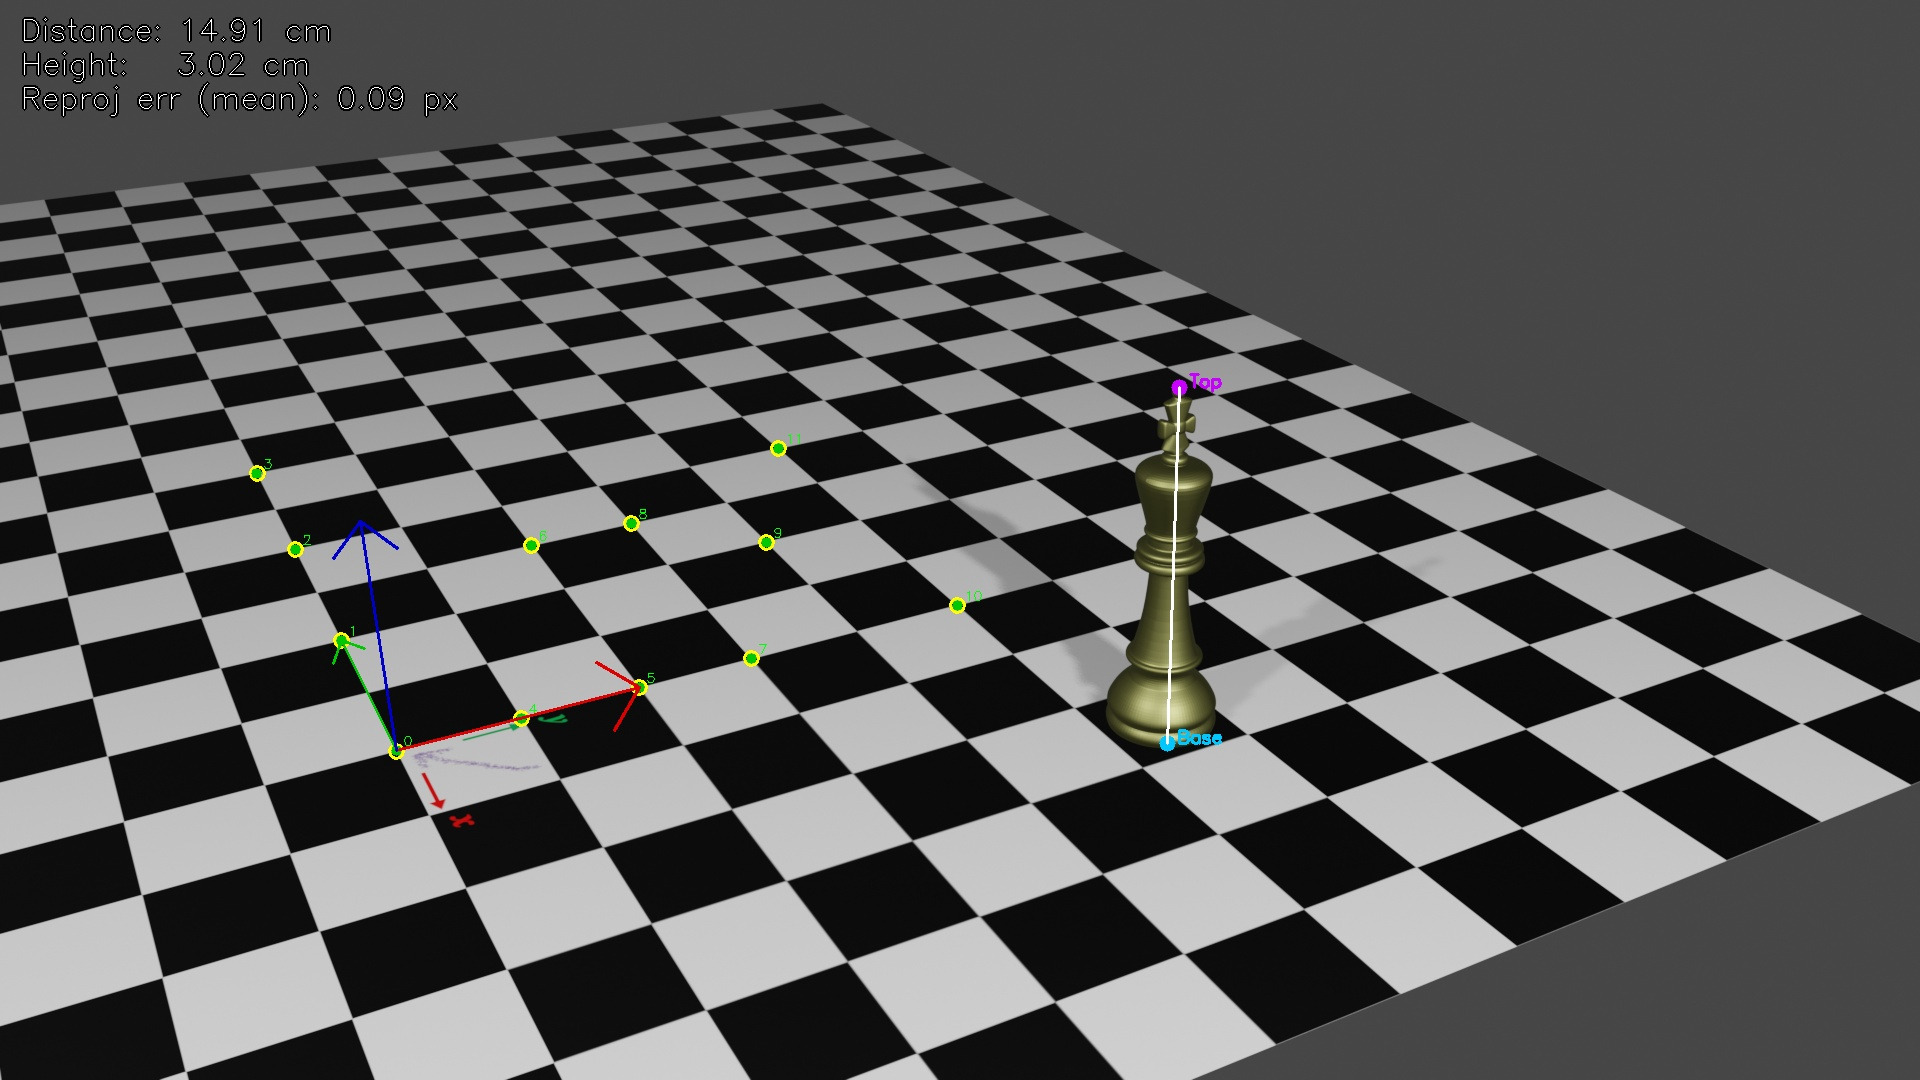
\includegraphics[width=0.88\linewidth]{result.jpg}
  \caption{Annotated result. \textcolor{green}{Green}: reference corners.
           \textcolor{yellow}{Yellow}: reprojected positions.
           \textcolor{cyan}{Cyan}: piece base. \textcolor{magenta}{Magenta}: crown tip.
           White line: measured height. Axes: $+X$ red, $+Y$ green, $+Z$ blue.}
\end{figure}

% ─────────────────────────────────────────────────────────────────────────────
\section{Discussion}
% ─────────────────────────────────────────────────────────────────────────────

The $u$/$v$ formula discrepancy (1.81 vs.\ 3.02 cm) is geometric, not numerical: the crown cross bar makes the topmost visible pixel laterally offset from the piece axis, and the $u$-formula's small denominator amplifies this into a $1.2\,\text{cm}$ bias. Primary error sources: (1) base pixel selection ($\pm2\,\text{px}\to\pm0.1\,\text{cm}$ distance); (2) corner detection ($<0.21\,\text{px}$ reprojection error); (3) crown tip pixel ($\pm1\,\text{px}\to\pm0.009\,\text{cm}$ height via $v$-formula). Camera elevation $C_Z=8.00\,\text{cm}$ yields elevation angle ${\approx}32.5°$ — consistent with the image perspective, confirming the pose estimate.

\end{document}
